\chapter{RADIOASTRONOMISKO DATU NOVĒROJUMU APSTRĀDES METODIKA}

Ventspils Starptautiskais Radioastronomijas Centrs ar kosmosa objektu novērošanu radio frekvenču diapazonā nodarbojas jau vairāk kā 10 gadus, bet tikai pēdējā gaida laikā VSRC pētnieki veic komētu novērojumus, kas sevī ietver komētas kodolā izveidojušo OH māzeru novērojumus. Bakalaura darba ietvaros tika izveidota metodika, kuras process atspoguļots \ref{fig:workflow} attēlā, kuru izmantojot ir iespējams apstrādāt iegūtos OH māzeru novērotos datus. Tiek arī apskatīti komētu novērojumu veikšanas kritēriji, piemēram, redzamības noteikšanas virs horizonta, objekta spilgtums un citi kritēriji.

%Lai gan VSRC pirms bakalaura darba izveides netika novēroti OH māzeri komētās, tiek veikti māzeru novērojumi citos radioastronomiskos objektos, taču metodika, ar kuru tiek novēroti šie objekti ir paredzēta spēcīgiem avotiem un avotiem ārpus Saules sistēmas. Līdz ar to, lai novērotu OH māzerus komētās Saules sistēmā, kā arī citos vājos objektos, tiek piedāvāta attēlā \ref{fig:workflow} aprakstītā metodika.

\begin{figure}[H]
\centering
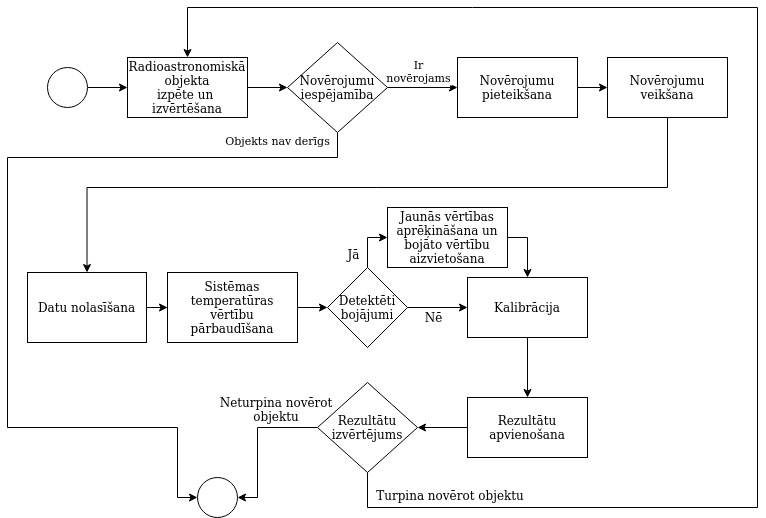
\includegraphics[width=\textwidth]{images/created/workflow-model.png}
\caption{Novērojumu apstrādes metodikas modelis}
\label{fig:workflow}
\end{figure}

%\begin{figure}[htbp]
%  \centering
%    \includesvg[width=\textwidth]{images/created/workflow.svg}
%  \caption{svg image}
%\end{figure}


Bakalaura darba ietvaros tiek aprakstīti visi soļi, izņemot \textit{Novērojumu pieteikšanas} un \textit{Novērojumu veikšanas} soļi, jo minētie soļi ir aprakstīti VSRC un Ventspils Augstskolas nolikumos un iekšējos dokumentos. Visi pārējie soļi aprakstīti pēc sekojošās metodikas - aprakstot teorētisko pamatojumu, realizāciju un iegūtos rezultātus. Radioastronomiskā objekta izpēte un izvērtēšana tiek apskatīta nodaļā \ref{planning}, kur tiek apskatīti raksturlielumi objekta novērošanā, kā arī teorētiskais apraksts novērojumu plānošanai.

Datu nolasīšanas sadaļa aprakstīta nodaļā \ref{read-data}, sistēmas temperatūras pārbaudes aprakstītas anomāliju detektēšana nodaļā \ref{anomalies}, bet pats kalibrācijas process aprakstīts \ref{calibration} nodaļā. Minēto soļu praktisku piemēru var apskatīt \ref{data-process} sadaļā. Novērojumu apvienošanas matemātiskais process aprakstīts \ref{doppler} nodaļā, bet radioastronomisko datu apstrādes rezultātus var apskatīt nodaļā \ref{result-eval}

\section{Novērojuma plānošanas process} \label{planning}



Lai veiktu radioastronmiskā objekta novērošanu, ir jāņem vērā vairāki faktori, kas ietekmēs rezultātu precizitāti un iespējamību. Lai gan turpmāk aprakstītās nodaļas novērojumu veikšanas kritēriji ir svarīgi, jāņem vērā, ka komētu, kuras iespējams detektēt radio frekvenču diapazonā, ir salīdzinoši maz, balstoties uz to, ka komētu OH māzeri izstaro vājus signālus, salīdzinot ar citiem OH māzeriem, līdz ar to ir ieteicams novērot visas komētas, kuras potenciāli detektējamas. Balstoties uz to, ka komētas daļēji sastāv no ledus maisījumiem, novērojumi var sniegt informāciju par ūdeni kosmosā, kā arī ūdens rašanos uz Zemes. Komētu sastāva izpēte sniedz vairāk informāciju komētu zinātniskajai bāzei, tajā skaitā, informāciju par ūdens rašanos uz Zemes, jo komētu sastāvā ir sastopams ūdens ledus formā. 

\begin{wrapfigure}{l}{0.4\textwidth}
    \centering
    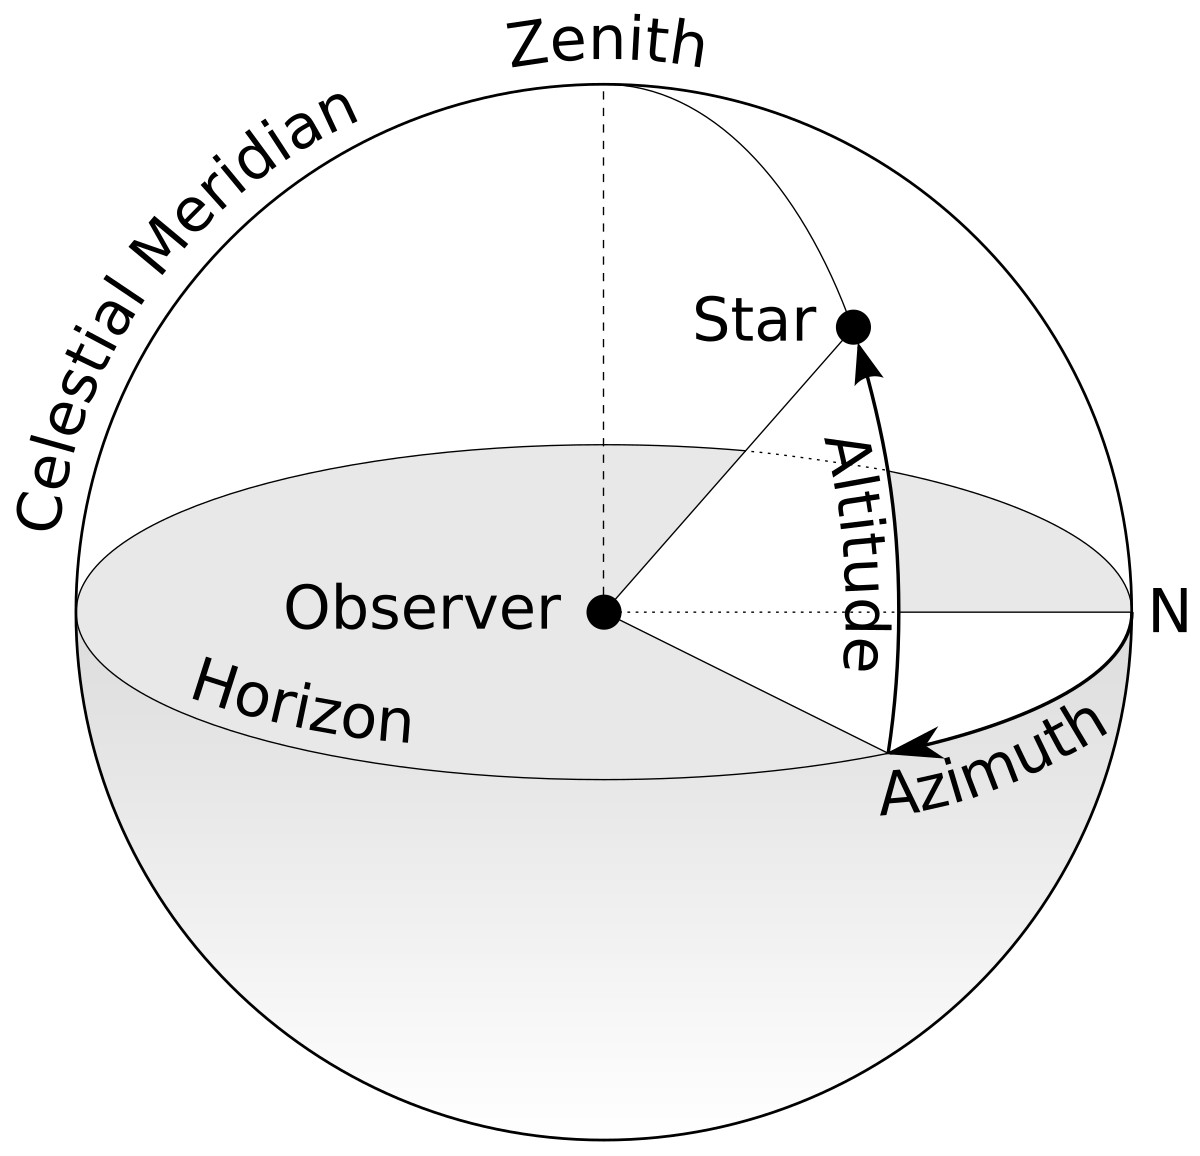
\includegraphics[width=0.4\textwidth]{images/internet/az-el.png}
    \caption{Topocentriskās koordinātu sistēmas attēlojums \cite{az-el-img}}
      \label{fig:az-el}
\end{wrapfigure}
 Par svarīgāko faktoru komētas detektēšanai ar radioteleskopu var uzskatīt objekta pozīciju. Astronomijā tiek izmantota topocentriskā koordināšu sistēma, kurā ir divas neatkarīgas lenķiskās koordinātes - azimuts un elevācija. Sistēma attēlota attēlā \ref{fig:az-el}, kur azimuts - Azimuth, bet elevācija - Altitude. Attēlā, objekts ir zvaigzne, bet zvaigznes vietā var būt jebkurš astronomisks objekts, kurš izstaro radio signālu. Bakalaura darba ietvaros izmantotais Irbenes RT-32 teleskops spējīgs novērot objektus rotējot 360 grādu leņķī, līdz ar to vienīgās vērtības, kuras jāņem vērā, lai novērojums būtu iespējams, ir elevācijas vērtība. Lai gan pēc radioteleskopa lietošanas specifikācijas minimālā elevācijas vērtība ieņem 2.7 grādu vērtību \cite{telescope-spec}, praksē pierādījies, ka elevācijas vērtībām jāpārsniedz 15 grādu robežām, lai iegūtais rezultāts būtu izmantojams, jo objektu novērošana tuvu horizontam nozīmē, ka tiek pastiprināti uztverti apkārtējie radio signālu avoti, kas atrodas uz Zemes virsmas, kā mobilie torņi, Ovīšu bāka un citi. Novērojumu sesijas ilgst vismaz 2 stundas, līdz ar to ir jāpārliecinās, ka elevācijas vērtības ir derīgas visa novērojuma laikā. 
 
 Objekta redzamības grafiku var apskatīt attēlā \ref{fig:swan-el}, kur apskatīts SWAN C/2020 F8 komētas elevācijas vērtības atkarībā no radioteleskopa un objekta pozīcijas no 1. maija līdz 10. maijam, ar sarkanu krāsu iezīmējot potenciāli iespējamos novērojumu laikus.\footnote{Elevācijas vērtības iegūtas no NASA HORIZONS sistēmas} ATLAS komētas redzamības grafiku skatīt pielikumā \ref{fig:atlas-visibility}. Visi grafiki nodaļā tiek izveidoti, izmantojot \textit{Matplotlib Python} bibliotēku \cite{matplotlib}. 

\begin{figure}[H]
\centering
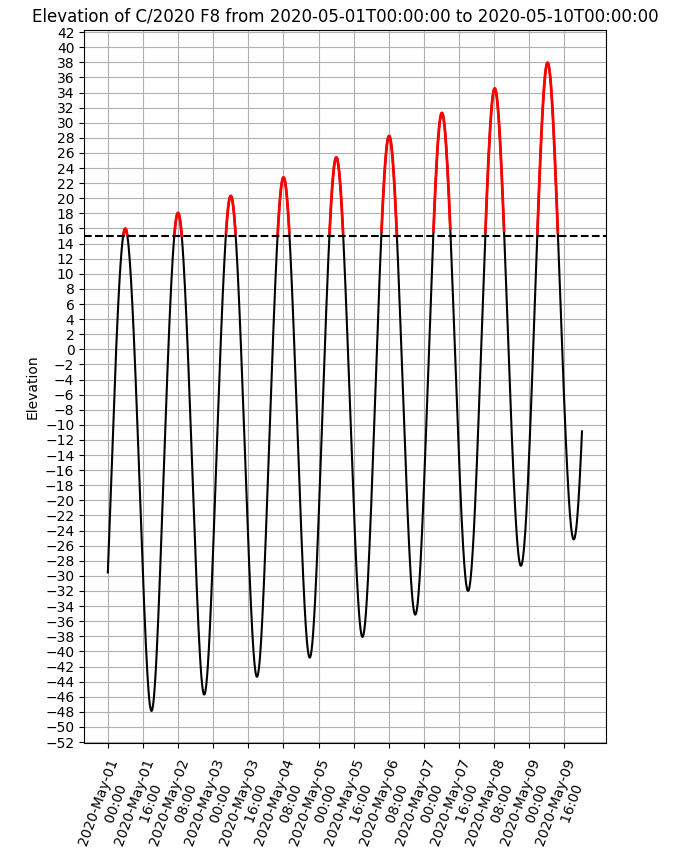
\includegraphics[width=0.75\textwidth]{images/created/swan-smaller.png}
\caption{SWAN C/2020 F8 elevācijas atkarība no laika}

\label{fig:swan-el}
\end{figure}



Veicot vāju radioastronomisku objektu novērojumus, ir nepieciešams novērojuma sesijas laikā novērot arī kādu spēcīgāku avotu jeb kalibratoru, kuru izmanto kontrolei. Tas nozīmē, ka arī kalibratoram ir jābūt redzamam sesijas laikā. Pēdējais nosacījums, objektu novērošanas iespējamībai fiziskā līmenī, ir radioteleskopa noslogojums. Ņemot vērā, ka uz teleskopa izmantošanu ir pieteikušies gan VSRC zinātnieki, gan citu valstu astronomisko institūtu zinātnieki, ir jāņem vērā citu zinātnieku vēlmes un jāplāno savstarpēji vislabākie laiki. 

Komētu datu kvalitāti ļoti ietekmē komētas spilgtums. 
Balstoties uz to, ka komētas aktīvi tiek novērotas optiskajā diapazonā, komētu spilgtums bieži tiek mērīts magnitūdās, pēc kurām iespējams novērtēt komētas spektrālo plūsmas blīvumu novērojumos radio diapazonā. Komētu spilgtumu precīzi noteikt nav viegli, taču izmantojot vairākus avotus, var iegūt aptuveno objekta spilgtumu magnitūdu skaitu. 
Katra magnitūda atbilst 2.512 spilgtuma faktoram, kas nozīmē, ka 1 magnitūdas spilgtuma objekts ir aptuveni 100 reizes spilgtāks par 6 magnitūdas spilgtuma objektu. Bakalaura darba ietvaros tika novērotas komētas, kuru aprēķinātais spilgtums svārstījās robežās no 12 līdz 4 magnitūdām.\footnote{Spilgtuma vērtības iegūtas no NASA HORIZONS sistēmas}

Viens no noteicošajiem faktoriem komētu novērošanas procesā ir komētas pārvietošanās pa tās orbītas. Lai veiksmīgi iegūtu augstas kvalitātes rezultātus, izmantojot patreizējās tehnoloģijas, ir nepieciešams novērot objektu ilgstošā laika periodā. Novērošanas ilgums katrai komētai atšķiras, balsoties uz tās strukturālajiem parametriem un orbītas, pa kuru komēta pārvietojas, taču Bakalaura darba izstrādes laikā, galvenajām novērotajām komētām, minimālais novērojumu laiks bija 110 stundas. Pilnus novērojumu laikus, kā arī citu informatīvo informāciju var apskatīt tabulā  \ref{tab:main-objects}.

Komētai tuvojoties Saulei, palielinās Saules ietekme uz komētu, kas izraisa ķīmiskas reakcijas komētas iekšienē. Komētai ir kodols, kas sastāv no $H_2O$ un papildus ķīmisko elementu piemaisījumiem. Miera stāvoklī kodols ir neaktīvs un sasalis, bet komētai tuvojoties Saulei, Saules ultravioletais starojums ietekmē kodolu. Kodols tiek aktivizēts un tā iekšienē veidojās OH māzeris, kas izstaro OH molekulas. Minēto starojumu ir iespējams novērot radio diapazonā. Kodola aktivitāte ir proporcionāla starojuma spilgtuma jaudai.


Veicot novērojumu, nepieciešams ņemt vērā arī novērotā objekta pozīciju attiecībā pret Zemi. Ņemot vērā, ka OH māzera izstarotais signāls ir salīdzinoši vājš, situācijās, kad komēta ir aktīva, taču atrodas tālu prom no Zemes, nav iespējams objektu novērot citu objektu izstaroto radio starojuma dēļ. Pēc teorijas, radioteleskops spējīgs novērot avotus tūkstošiem astronomisko vienību attālumā, pieņemot, ka avots ir pietiekami spēcīgs. Praksē pierādījies, ka komētām jābūt maksimāli divu astronomisko vienību attālumā no novērošanas punkta, kur komēta, ideālā gadījumā, novietota starp Zemi un Sauli.

Neskatoties uz precīziem skaitļiem, ir jāņem vērā arī komētas popularitāte starp citiem novērotājiem. Jo vairāk astronomi novēro vienu objektu, jo vairāk informācijas pieejama, tādējādi radot iespēju salīdzināt iegūtos rezultātus, kā arī no vairākiem novērojumiem ir efektīvāk iespējams uzzināt objekta aktualitātes. Lai gan pārsvarā astronomi novēro komētas optiskajā diapazonā, rezultāti sniedz informāciju par komētas izmaiņām, piemēram, pateicoties minēto avotu informācijai, bija iespējams detektēt ATLAS Y4/2019 kodola fragmentāciju, kas ļoti ietekmē novērošanas plānus.



%\section{Kopējais process (Workflow)}
\section{Datu nolasīšana} \label{read-data}
% intro
Lai uzsāktu datu apstrādi, ir nepieciešams vispirms izprast datu tipa uzbūvi. Bakalaura darbā tiek apskatīti divi datu tipi, kuri izmantoti komētu novērojumu datu ieguvē un izguvē - jēldati un dat tipa faili. Nodaļā tiks aprakstīta atšķirība starp tiem, kā arī apstrādes process datu izmantošanai.

%novērojumu datu struktūra
%Katrs novērojuma skans ir sadalīts 


% RAW

Katrs novērojuma skans jēldatu gadījumā ir sadalīts astoņās atsevišķās datnēs, kur katrā ir ierakstīts spektrs \textit{int16+int16} reālu un imagināru skaitļu virknē. Lai nolasītu datus, pēc \textit{SDR} spektometra servera dokumentācijas \cite{sdrspec}, Bakalaura darba rakstīšanas laikā visai jēldatu apstrādei papildus Furjē transformācijai, jāizmanto \textit{Blackman-Harris} logošanas funkcija \cite{blackman-harris}, lai iegūtu rezultējošu spektru. Balstoties uz to, ka ieteiktā pārklāšanās robeža \textit{Blackman-Harris} funkcijai ir 66.1\% \cite{overlapping}, tika izveidots algoritms, kas sadala nolasītos datus tvertnēs, kuru garums ir identisks žurnalēšanas failu ierakstītajai \textit{Ns} vērtībai.

Katrai tvertnei tiek izsaukta \textit{Fast Fourier Transform} (turpmāk FFT), kā arī Blackman-Harris funkcija. FFT realizēta, izmantojot \textit{numpy FFT} pakotni \cite{numpy-fft}, bet Blackman-Harris logošanas funkcija izmantojot \textit{scipy signal} pakotni \cite{scipy-blackman}. Pēc FFT veikšanas, tiek apvienotas spektra reālās un imaginārās daļas, un rezultāts ir pieskaitīts kopējai spektru summai. Kad visas datu tvertnes ir apstrādātas, nulles frekvences ir pārvietotas uz vidu un rezultējošais spektrs ir izdalīts ar tvertņu daudzumu, iegūstot vidējo spektru, kas ir skaitļu masīvs ar amplitūdu vērtībām, kuras iegūtas no konkrētā faila. Vizuāli process izklāstīts attēlā \ref{fig:overlapping}, kur attēlots pārklāšanās process izmantojot 75\% pārklāšanās koeficientu. Lai gan attēlā attēlots 75\% pārklāšanās rezultāts, datu apstrāde ar 66.1\% pārklāšanās koeficientu ir ļoti līdzīga, jo mainās tikai kopējais spektru daudzums.

\begin{figure}[H]
\centering
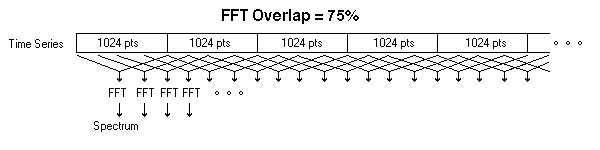
\includegraphics[width=\textwidth]{images/internet/OVERLAP2.png}
\caption{Furjē transformācijas pielietojums uz datu tvertnēm ar 75\% pārklāšanās koeficientu. \cite{overlapping-img}}
\label{fig:overlapping}
\end{figure}

% DAT
Dat formāta datu gadījumā, dati jau ir apstrādāti ar iepriekš minētajām funkcijām, līdz ar to tie ir ierakstīti \textit{CSV} tipa failā trijās kolonnās. Pirmajā kolonnā ierakstītas frekvenču joslas vērtības konkrētajām amplitūdām, otrajā kolonna ierakstītas kreisās cirkulārās polarizācijas amplitūdu vērtības, bet trešajā ierakstītas labās cirkulārās polarizācijas amplitūdu vērtības. Tā kā abas polarizācijas ir saglabātas vienā failā, kopējais failu daudzums vienam skanam ir četri.

Kopējais failu skaits novērojumā atkarīgs no novērojuma ilguma, taču katram failam nav precīza ierakstīšanas ilguma. Četru stundu novērojumiem kopā ir 240 skani, bet divu stundu novērojumiem 120. Balstoties uz minēto informāciju, var detektēt situācijas, kur novērošanas sesijā bijušas tehniskas problēmas, jo patiesais failu daudzums neatbilst plānotajam, un izvērtēt, vai datus izmantot.

Lai gan dat formāta failu rezultāti ir neprecīzāki par jēldatu failu rezultātiem, tie tiek biežāk izmantoti sava ērtuma dēļ, jo bieži tiek apskatīti spēcīga signāla objekti un noklusējuma konfigurācija tiem ir apmierinoša. Priekšrocība jēldatiem ir to konfigurēšanas iespējas, taču jāņem vērā, ka to apstrādei nepieciešami vairāk skaitļošanas un laika resursi. Novērojot objektus un rezultātus ierakstot jēldatu formātā,  nepieciešama salīdzinoši liela datu krātuve, jo divu stundu novērojums atbilst aptuveni 340 gigabaitiem atmiņas, kamēr dat tipa failu novērojumi aizņem tikai ap 70 megabaitiem.

Lai izvērtētu datu apstrādes veiktspēju, tiek veikti veiktspējas testi, kuri aprakstīti \ref{algorithm-eval} nodaļā, kur apskatīts gan pirmās iterācijas, gan pēdējās iterācijas algoritmu izpildes laiks, kā arī procesu daudzuma ietekme uz pēdējās iterācijas algoritma izpildes laiku. Algoritma realizāciju var apskatīt pielikumā \ref{appendix:codes}.

% comparison?
%Nodaļai nevar būt tikai viena apakšnodaļa. Analītiskās daļas  uzdevums ir sistematizētā veidā sniegt pētāmās problēmas īsu teorētisku pamatojumu, autora pētījuma rezultātus, kas formulēti priekšlikumu veidā. Visās analītiskās daļas nodaļās (izņemot teorētisko pamatojumu) jābūt ilustratīvajam materiālam un aprēķiniem: konkrētiem plāna aprēķiniem, analītiskām tabulām, diagrammām u.tml.


\section{Kalibrācijas process} \label{calibration}

%pamatojums, kāpēc kalibrācija ir nepieciešama

% galvenās darbības kaliobrācijas procesā
%% formulas arī
%piezīmei par kalibrācijas uzlabojumi tiks apskatītiti ndoaļa 3.2.xxx

Nodaļā aprakstītas kalibrācijas procesā izmantotās formulas, taču ņemot vērā, ka Bakalaura darba mērķis ir orientēts uz algoritmisko izpildi, nevis fizikālo pamatojumu, formulu izmantošanas pamatojums netiek sniegts. Aprakstītā kalibrācijas metode tiek izmantota spēcīgu māzeru novērojumos, līdz ar to, pamatalgoritms ir ticis izveidots jau iepriekš, ņemot par pamatu citās radio stacijās izmantotos kalibrēšanas algoritmus.

Kalibrācijas process ir izveidots, izmantojot rakstu \textit{Unbiased flux calibration methods for spectral-line radio observations} \cite{unbiased}, kurā aprakstītas metodes efektīvai datu kalibrācijai - pozīciju maiņa un frekvenču maiņa. Pozīciju maiņā teleskops tiek norādīts uz references pozīciju pirms tas tiek pozicionēts uz novērojumu objektu.
Frekvenču maiņas metodē, tiek izmantoti divi lokālie oscilatori, kur viens no tiem tiek izmantots, lai sniegtu atskaites spektru. Veicot novērojumus teleskopa stars netiek fiziski bīdīts prom no avota, līdz ar to, nav iespējams veikt pozīciju maiņas pieeju, tāpēc tiek izmantota frekvenču maiņas metode.

Frekvenču maiņas metodes rezultātā veidojas 4 dažādas fāzes - $P_{off}^{sig}$, $P_{on}^{sig}$, $P_{off}^{ref}$, $P_{on}^{ref}$. Šie apzīmējumi tiek izmantoti formulās \eqref{eq:1.2.1}, \eqref{eq:1.2.2}, \eqref{eq:1.2.3}, \eqref{eq:1.2.4}, \eqref{eq:1.2.5} un \eqref{eq:1.2.6},
kur: 
\begin{tabbing}
\phantom{\hspace{10mm}}\= \kill
$P_{off}^{sig}$\> = Lokālā oscilatora ierakstītais signāls ar izslēgtu trokšņa diodi\\
$P_{on}^{sig}$\>   = Lokālā oscilatora ierakstītais signāls ar ieslēgtu trokšņa diodi\\
$P_{off}^{ref}$\>   = References lokālā oscilatora ierakstītais signāls ar izslēgtu trokšņa diodi\\
$P_{on}^{ref}$\> = References lokālā oscilatora ierakstītais signāls ar ieslēgtu trokšņa diodi\\
\end{tabbing}

Lai iegūtu datus par objekta plūsmas blīvumu, ir jāņem vērā kopējā sistēmas trokšņa temperatūra pēc formulas \ref{eq:1.2.1}. 

\begin{equation}
T_{sys}^{[cal]} = T_{bg} + T_{atm} + T_{atm} + T_{spill} + T_{loss} + T_{rx} + T_{cal} \tag{1.2.1}\label{eq:1.2.1} 
\end{equation}
kur: 
\begin{tabbing}
\phantom{\hspace{10mm}}\= \kill
$T_{sys}^{[cal]}$\> = Kopējā sistēmas trokšņa temperatūra \\
$T_{bg}$\> = Mikroviļņu un galaktiskā fona troksnis \\
$T_{atm}$\> = Atmosfēras troksnis \\
$T_{spill}$\> = Zemes virsmas troksnis \\
$T_{loss}$\> = Novērojumā zaudētā informācija \\
$T_{rx}$\> = Uztvērēja trokšņa temperatūra \\
$T_{cal}$\>   =  Injicētais troksnis, izmantojot trokšņa diodi\\
\end{tabbing}



Taču visas minētās vērtības iegūt nav vienkārši, līdz ar to tiek piedāvāts alternatīvs veids, kā aprēķināt sistēmas temperatūru no iegūtajiem datiem. Ja $T_{sys}^{off}$ un $T_{cal}$ tiek uzskatītas par konstantēm attiecībā pret laiku un frekvenci, iegūst vienādojumus:
%Eq25
\begin{equation}
T_{sys,ref}^{off} = T_{cal} \frac{ \left( P_{on}^{ref} + P_{off}^{ref} \right)  -  \langle P_{on}^{ref} - P_{off}^{ref} \rangle_v }{2 \langle  P_{on}^{ref} - P_{off}^{ref} \rangle} \tag{1.2.2}\label{eq:1.2.2} 
\end{equation}
kur: 
\begin{tabbing}
\phantom{\hspace{30mm}}\= \kill
$\langle P_{on}^{ref} - P_{off}^{ref} \rangle_v$\> = References oscilatora spektru starpības iekšējo 50 \% vidējā vērtība\\
$T_{cal}$\>   =  Injicētais troksnis, izmantojot trokšņa diodi\\
$T_{sys,ref}^{off}$\> = Sistēmas temperatūra izslēgtai trokšņa diodes references oscilatora signālam\\
\end{tabbing}

\begin{equation}
T_{sys,sig}^{off} = T_{cal} \frac{ \left( P_{on}^{sig} + P_{off}^{sig} \right)  -  \langle P_{on}^{sig} - P_{off}^{sig} \rangle }{2 \langle  P_{on}^{sig} - P_{off}^{sig} \rangle} \tag{1.2.3}\label{eq:1.2.3} 
\end{equation}
\begin{tabbing}
\phantom{\hspace{30mm}}\= \kill
$\langle P_{on}^{sig} - P_{off}^{sig} \rangle_v$\> = Lokālā oscilatora spektru starpības iekšējo 50 \% vidējā vērtība\\
$T_{cal}$\>   = Injicētais troksnis izmantojot trokšņa diodi\\
$T_{sys,sig}^{off}$\>  = Sistēmas temperatūra izslēgtai trokšņa diodes lokālā oscilatora signālam\\
\end{tabbing}
%EQ:24
%\begin{equation}
%\frac{T_{sys,off}}{T_{cal}} \approx \frac{(P_{off}^{cal}+P_{off}) - \langle P_{off}^{ref} - P_{off}^{ref}\rangle_v }{2 \langle  P_{off}^{cal}-P_{off} \rangle_v }
%\end{equation}





%EQ27:

%\[T_{sou} = \overline{T}_{sys,off} \frac{P_{on} - P_{off}{4} \]

%article formula:
%\[ T_{sou} = \overline{T}_{sys,off} \frac{P_{on}-P_{off}}{P_{off}} = \left( \overline{T}_{sys,off} + T_{cal} \right) \frac{P_{on}^{cal} - P_{off}^{cal}}{P_{off}^{cal}} \]

Izmantojot skalāru $T_{cal}$ vērtību, zināmu katram uztvērējam, var iegūt kalibrētu spektru izslēgtai trokšņa diodei:

\begin{equation}
T_{cal,ref}^{off} = T_{sys,ref}^{off} \cdot \frac{(P_{off}^{sig} - P_{off}^{ref})}{P_{off}^{ref}}\tag{1.2.4}\label{eq:1.2.4} 
\end{equation}
kur:
\begin{tabbing}
\phantom{\hspace{20mm}}\= \kill
$T_{sys,ref}^{off}$\>  = Sistēmas temperatūra izslēgtai trokšņa diodes references oscilatora signālam\\
$T_{cal,ref}^{off}$\>  = Kalibrētas sistēmas temperatūra izslēgtai trokšņa diodes references oscilatora \\ signālam\\
\end{tabbing}
\begin{equation}
T_{cal,sig}^{off} = T_{sys,sig}^{off} \cdot \frac{(P_{off}^{ref} - P_{off}^{sig})}{P_{off}^{sig}}\tag{1.2.5}\label{eq:1.2.5} 
\end{equation}
kur:
\begin{tabbing}
\phantom{\hspace{20mm}}\= \kill
$T_{sys,sig}^{off}$\>  = Sistēmas temperatūra izslēgtai trokšņa diodes lokālā oscilatora signālam\\
$T_{cal,sig}^{off}$\>  = Kalibrētas sistēmas temperatūra izslēgtai trokšņa diodes lokālā oscilatora \\ signālam\\
\end{tabbing}

Līdz ar to, lai aprēķinātu sistēmas temperatūru ieslēgtai trokšņa diodei, papildus jāapskata trokšņa diodes temperatūra. 
%34

\begin{equation}
T_{cal,ref}^{on} = \left( T_{sys,ref}^{off} + T_{cal} \right) \cdot \frac{\left( P_{on}^{sig} -  P_{on}^{ref}\right)}{ P_{on}^{ref}}\tag{1.2.6}\label{eq:1.2.6}   
\end{equation}

\begin{equation}
T_{cal, sig}^{on} = \left( T_{sys,sig}^{off} + T_{cal} \right) \cdot \frac{\left( P_{on}^{ref} -  P_{on}^{sig}\right)}{ P_{on}^{sig}}\tag{1.2.7}\label{eq:1.2.7}  
\end{equation}
kur:
\begin{tabbing}
\phantom{\hspace{20mm}}\= \kill
$T_{cal,ref}^{on}$\>  = Rezultējošā sistēmas temperatūra lokālā oscilatora references signālam\\ ieslēgtai trokšņa diodei\\
$T_{cal,sig}^{on}$\>  = Rezultējošā sistēmas temperatūra lokālā oscilatora signālam ieslēgtai \\ trokšņa diodei\\
$T_{sys,ref}^{off}$\>  = Kalibrētas sistēmas temperatūra izslēgtai trokšņa diodes lokālā oscilatora \\ signālam izslēgtai trokšņa diodei\\
$T_{sys,ref}^{off}$\>  = Kalibrētas sistēmas temperatūra izslēgtai trokšņa diodes lokālā oscilatora \\references signālam \\
$T_{cal}$\>  = Injicētais troksnis, izmantojot trokšņa diodi\\


\end{tabbing}

%\[ T_{sou,-} - T_{sou,+} + \Delta T_{sys,\pm}^{[cal]} = \left( T_{sou,-} + T_{sys,-}^{[cal]}  \right) \frac{P_{ref}^{[cal]}-P_{ref}^{[cal]}}{P_{sig}^{[cal]}} \equiv \Tilde{T}_{ref}^{[cal]} \]

Spektri ir apvienoti, lai gala rezultātā samazinātu troksni:

\begin{equation}
T_{cal}^{sig} = \frac{T_{cal, sig}^{on} + T_{cal, sig}^{off}}{2} \tag{1.2.8}\label{eq:1.2.8} 
\end{equation}

\begin{equation}
T_{cal}^{ref} = \frac{T_{cal, ref}^{on} + T_{cal, ref}^{off}}{2}\tag{1.2.9}\label{eq:1.2.9} 
\end{equation}


Lai iegūtu optimālu rezultātu $T_{rez}$ vērtības, ir arī jāveic frekvenču pārvirzīšana, bet Bakalaura darba ietvaros tiek izmantota \textit{ numpy roll } funkcija, kurai tiek padots $T_{rez}$ spektrs, kā arī pārbīdes koeficients. Rezultējošie spektri tiek apvienoti:
\begin{equation}
T_{rez} = \frac{T_{cal}^{sig} + T_{cal}^{ref}}{2}\tag{1.2.10}\label{eq:1.2.10} 
\end{equation}


Rezultāti tiek pārveidoti no kelviniem uz janskijiem, lai efektīvāk attēlotu plūsmas blīvumu. Jāņem vērā Zemes atrašanās vieta attiecībā pret objektu, līdz ar to tiek rēķinātas vērtības polinoma vērtības Zemes atrašanās vietā. Tas tiek darīts pēc formulas:

\begin{equation}
Sf = \frac{T_{rez}}{ DPFU \cdot f(Gel,El))}\tag{1.2.11}\label{eq:1.2.11} 
\end{equation}
kur:
\begin{tabbing}
\phantom{\hspace{30mm}}\= \kill
$Sf$\>  = Rezultējošais spektrālās plūsmas blīvums\\
$T_{rez}$\>  = Rezultējošā sistēmas temperatūra\\
$DPFU$\>  = (Degree per flux unit) Grādi uz plūsmas vienību\\
$f(Gel,El))$\>  = Aprēķinātā elevācijas polinoma vērtība \\
\end{tabbing}

Nodaļā aprakstītās formulas tiek pielietotas divreiz, katrai polarizācijai.
Kalibrācijas rezultātā tiek iegūts plūsmas blīvuma spektrs, kurš attēlo enerģiju, kas iegūta attālumā no novērotā objekta laukuma, kurš atrodas novērojuma brīdī veiktajā attālumā starp radioteleskopu un novēroto objektu. Algoritma implementāciju var apskatīt pielikumā \ref{appendix:codes}.



\section{Doplera kompensācija un objekta pārvietošanās ātruma aprēķins} \label{doppler}
Nākamais solis vāju radioastronomisku objektu novērojumu procesā ir vairāku novērojumu apvienošana. Ņemot vērā, ka katrā novērojuma iterācijā stohastiskais troksnis dod signālam dažādas vērtības, apvienojot vairākus novērojumus, stohastiskais troksnis samazināsies ar katru iterāciju, bet novērojuma objekta vērtības nemainīsies.  Lai to realizētu, ir jāņem vērā faktors, ka gan novērotais objekts, gan Zeme pārvietojas Saules sistēmā. Tas nozīmē, ka rezultējošo novērojuma frekvenci ietekmēs Doplera efekts un iegūtais frekvenču masīvs ir jāmodificē, lai pārbīde tiktu ņemta vērā. 

Doplera efekta aprēķins ir atšķirīgs, atkarībā no objekta atrašanās vietas. Ņemot vērā to, ka Bakalaura darba ietvaros, tika apskatīti gan Saules sistēmas objekti, gan maiņzvaignes un māzeri ārpus Saules sistēmas, tika izpētītas atšķirīgās pieejas nobīdes aprēķinam. Lai aprēķinātu Doplera efektu objektiem ārpus Saules sistēmas, ir nepieciešams zināt objektu pārvietošanās ātrumu. Tā kā novērotos radioastronomiskos objektus ārpus Saules sistēmas var uzskatīt par punktveida objektiem, visa ātruma vektoru ietekme tiek aprēķināta ar formulu:
\begin{equation}
V_{total} = (V_{sun} + V_{obs} + V_{Earth}) \tag{1.3.1}\label{eq:1.3.1} 
\end{equation}
kur: 
\begin{tabbing}
\phantom{\hspace{10mm}}\= \kill
$V_{total}$\> = Rezultējošais objekta ātrums \\
$V_{sun}$\>   = Vidējais Saules pārvietošanās ātrums novērojuma laikā\\
$V_{obs}$\>   = Vidējais objekta ātrums novērojuma laikā\\
$V_{Earth}$\> = Vidējais Zemes pārvietošanās ātrums novērojuma laikā\\


\end{tabbing}



Lai iegūtu rezultējošās objekta pārvietošanās ātruma vērtības, tika izmantots jau eksistējošs programrisinājums, kas tika radīts radioastronomisku māzeru novērojumiem.\cite{vlsr} %mention RA/DEC? 
Metode izmanto māzera spektrālo līniju pīķus, lai iegūtu rezultējošo ātrumu pēc formulas:


\begin{equation}
V_{rez}=\left(\frac{f_{obs}}{f_{rest}}-1 \right) \cdot c + V_{total} \tag{1.3.2}\label{eq:1.3.2} 
\end{equation}
kur: 
\begin{tabbing}
\phantom{\hspace{10mm}}\= \kill
$V_{rez}$\> = Rezultējošais ātruma masīvs, attiecīgajai frekvencei \\
$f_{obs}$\>   = Novērojumā iegūtā frekvenču josla\\
$f_{rest}$\>   = OH molekulu spektrālo līniju frekvence \\
$c$\> = Gaismas ātrums\\
$V_{total}$\> = Objekta rezultējošais pārvietošanās ātrums (skat. \eqref{eq:1.3.1} formulu) \\\\

\end{tabbing}

Ķermeņus Saules sistēmā nevar uzskatīt par punktveida objektiem, jo ātruma vektoru ietekme uz objektu ir lielāka. Lai iegūtu radioastronomiskā objekta ātrumu, ir iespējams izmantot Keplera orbitālos parametrus \cite{kepler-elements}, taču lai atvieglotu darbu, kā arī mazinātu kļūdu iespējamību, tiek izmantota NASA HORIZONS sistēma \cite{horizons}, kura uzglabā lielu daudzumu informācijas par Saules sistēmas objektiem, to skaitā, objektu atrašanās vietu konkrētos laikos, kā arī objektu ātrumu konkrētajā laikā. Iegūtais ātrums novērojuma laika periodā tiek ievietots \eqref{eq:1.3.2} formulas $V_{total}$ mainīgajā.


Novērojumu veikšanas laikā, Doplera pārbīde jau tiek ņemta vērā, izmantojot aprakstīto metodiku, taču esošais algoritms paredzēts mazāka joslas platuma novērojumos, līdz ar to tiek izmantots vidējais ātrums visā novērojumā. Ņemot vērā minēto faktoru, spektrs tiek pārbīdīts atpakaļ par nobīdīto vērtību, sadalīts uz pusēm, kur pirmā puse reprezentē 1665MHz frekvences diapazona spektru, bet otra puse - 1667MHz frekvences diapazona spektru, katrai daļai pārrēķinātas ātruma vērtības un attiecīgi pārbīdītas. Pareizā pārbīde tiek rēķināta pēc formulas:


\begin{equation}
df  = f_0 - \frac{f_0}{1- \frac{V_{object}}{c}}
\tag{1.3.3}\label{eq:1.3.3} 
\end{equation}
kur: 
\begin{tabbing}
\phantom{\hspace{15mm}}\= \kill
${df}$\> = Aprēķinātā spektra nobīde \\
$f_{0}$\>   = Novērojumā iegūtā frekvenču josla\\
$c$\> = Gaismas ātrums\\
$V_{object}$\> = Objekta radiālais ātrums relatīvs uztvērēja antenai \\\\

\end{tabbing}





%vel = rezultējošais ātruma masīvs

%f_obs = frekvenču masīvs, kurš iegūts kalibrācijas rezultātā

%f_rest = rest frekvence (1.665402 vai 1.6673590) 

%c = gaismas ātrums

%v_sun = vidējais saules ātrums? vai šis būtu VmagSn no HORIZONS? (Magnitude of target center velocity with respect to the Sun)

%v_obs = objekta ātrums? vai šis būtu VmagOb no HORIZONS?

%v_earth = vidējais zemes ātrums?

%v_total = ātrums, kuru lieku iekšā doplera funkcijā

%Piemēra rezultāti uz atlas 0:

%v_sun:  5.3263164389446

%v_obs:  0.08472007198849721

%v_earth:  -15.215724915542548

%v_total:  -9.80468840460945




\section{Veivletu izmantošana radioastronomisku signālu apstrādē} \label{wavelets}
\subsection{Veivletu definēšana}
%pamatojuma daļā aprakstīt, ka veicletu teoretiskā ... netik plai izklāštīts, bet galvenasi uzsvars ir uz to izmantošanutiek izmantoti
Lai precīzāk analizētu signālus ar pēkšņām pārmaiņām, ir nepieciešams izmantot netradicionālākas metodes par Furjē transformāciju, kas reprezentē signālu kā sinosoīdu summu, kas nav lokalizēta laikā vai telpā. Lai veiktu signālu apstrādi, tika izmantota jauna funkciju klase – veivleti.  

Veivlets ir viļņveida svārstība ar amplitūdu, kas sākas ar nulli, palielinās vai samazinās un gala rezultātā atgriežas nulles vērtībā. Veivletiem ir dažādi tipi un grupējumi, un tos arī iedala pēc īpašībām, taču tiem ir vienots nosacījums -  veivleta amplitūdas vidējā vērtība ir nulle. Veivletu plašais formu klāsts ir viens no galvenajiem iemesliem veivletu izmantošanai signālu apstrādē. Lai vieglāk grupētu veivletus, tie ir iedalīti vairākās ģimenēs, taču konkrētie veivleti ir tikai visbiežāk izmantotie – veivletus var veidot jebkurš, ja vien izveidotais atbilst kritērijiem. 


Viena no veivletu transformācijas formām ir diskrētā vievletu transformācija, kura visbiežāk tiek izmantota datu trokšņa samazināšanā un datu kompresijā. Process ir līdzīgs signāla salīdzināšanai ar filtru bankām. Diskrētā veivletu transformācija attēlota attēlā \ref{fig:wavelets-dwt}, kur modelēts apstrādes process.

\begin{figure}[h!]
\centering
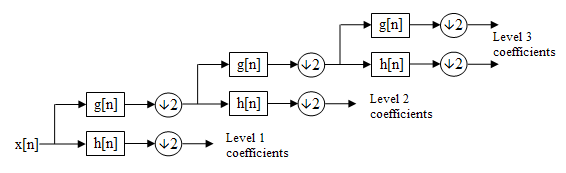
\includegraphics[width=\textwidth]{images/internet/DWT-fig.png}
\caption{Diskrētās veivletu transformācijas vizuālais attēlojums} \cite{dwt-fig}
\label{fig:wavelets-dwt}

\end{figure}



Signāls tiek filtrēts, izmantojot \textit{low-pass} un \textit{high-pass} filtrus, lai iegūtu \textit{low-pass} jeb aproksimācijas koeficientu, un \textit{high-pass} jeb detaļu koeficientu apakšjoslas. Nākamajā dekompozīcijas līmenī, \textit{low-pass} apakšjosla, tiek iteratīvi filtrēta, izmantojot to pašu metodi, kuru sākuma signāls. Koeficientu daudzums katrā apakšjoslā ir puse no koeficientiem no iepriekšējās apakšjoslas. 


Lai gan veivletiem ir vairākas metodes, kā tos pielietot signāla trokšņa samazināšanai, Bakalaura darba ietvaros tika izmantota veivletu sliekšņošna. Ir apskatītas diva veida slieksņošanas operācijas – mīkstā un cietā. Abos gadījumos koeficientiem ar vērtībām zem noteiktā sliekšņa tiek piešķirta vērtība nulle, bet atšķiras, kas notiek ar pārējiem koeficientiem. Mīkstajā metodē koeficienti, kas lielāki par norādīto slieksni ir samazināti, atņemot sliekšņa vērtību no koeficienta vērtības, taču cietajā – koeficienti paliek nemainīgi. Bakalaura darba ietvaros pēc noklusējuma tiek izmantota mīkstā sliekšņošanas metode, jo metodes pielietojums bija piemērotākā uzdevumu veikšanai.
%Vizuāli attēlojot šo procesu un apzīmējot high-pass apakš joslu ar h[n] un low-pass apakš joslu ar g[n], iegūst Ilustrāciju 1.  

%[bilde]



\subsection{Veivletu pielietojums}

Veivletu transformācija Bakalaura darba ietvaros tika realizēta izmantojot \textit{PyWavelets} \cite{pywt} Python bibliotēku. Bibliotēka tika izvēlēta, tās atvieglotās veivletu transformācijas realizācijas dēļ, kā arī plašo iebūvēto veivletu dēļ. Pēc noklusējuma tiek atbalstīti 106 veivleti, kuri atbalsta diskrēto veivletu transformāciju no sekojošām ģimenēm - bior, coif, db, dmey, haar, rbio, sym.

Plašo konfigurēšanas iespēju dēļ, veivletu pielietošana tika testēta gandrīz visos datu apstrādes procesos, ar atšķirīgu efektivitāti. Pielietojot šāda veida transformāciju, jāņem vērā, ka ar katru transformāciju, tiek zaudēti ar vien vairāk dati. Tas nozīmē, ka, ja transformācija tiks izmantota pārāk daudz, var tikt zaudētas spektra detaļas, kuras sākotnēji būtu redzamas. Arī jāņem vērā, ka iegūtais spektrs ir balstīts uz paša veivleta formu, līdz ar to, var rasties situācijas, kur veivlets izceļ pīķi konkrētā vietā, taču tas nav meklētais signāls. Problēma tiek novērsta salīdzinot vairāku veivletu iegūtos rezultātus savā starpā, jo, ja vairākas formas veivletu spektri iegūst pīķi vienādās frekvences vērtībās, var uzskatīt, ka tā nav sagadīšanās.

\begin{figure}[h!]

\centering
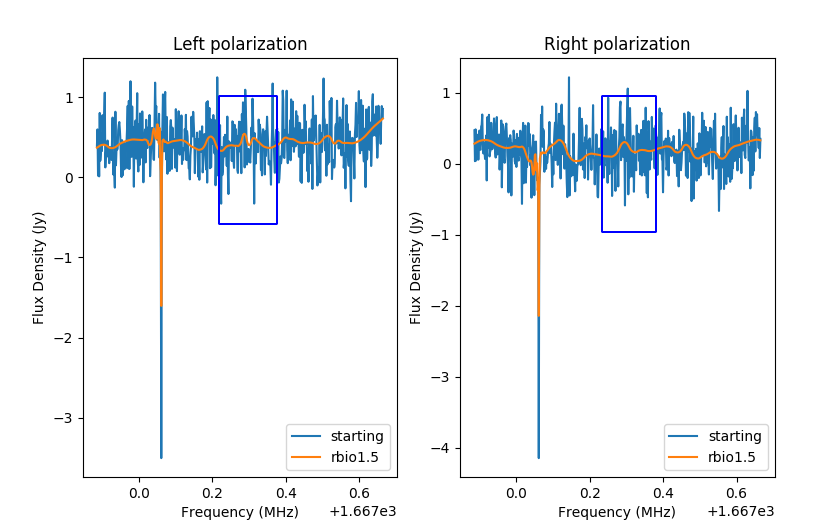
\includegraphics[width=\textwidth]{images/created/rbio15-rlmi-sdr-boxed.png}
\caption{Pirmie iegūtie rezultāti uz R Leonis Minoris izmantojot rbio1.5 veivletu ar 0.5 slieksni}
\label{fig:rlmi-boxed}
\end{figure}


Veivletu transformācijas pielietojuma iespējas ir ļoti plašas augstās konfigurēšanas iespējas dēļ, jo ir iespējams izmantot visus 106 iebūvētos veivletus un tiem norādīt savu precizitātes koeficientu, kā arī sliekšņošanas tipu. Tas nozīmē, ka katrs veivlets var tikt pielietots datiem, bet atkarībā no pielietotā veivleta rezultāts būs labāks vai sliktāks. Bakalaura darba pētījuma laikā tika atrasti vairāki veivleti, kurus iespējams efektīvi izmantot visos apskatītajos gadījumos.



Veivletu pielietošana Bakalaura darba ietvaros aizsākās ar mērķi novērst stohastisko troksni pirms vairāku novērojumu apvienošanas. Izmantojot veivletus, bija iespējams detektēt pirmās pazīmes maiņzvaigznes R Leonis Minoris OH māzera novērošanā, kuras attēlotas attēlā \ref{fig:rlmi-boxed}. Grafikā attēlota plūsmas blīvuma attiecība pret frekvenci, kur, izmantojot sākotnējo signālu, ir izveidots jauns spektrs izmantojot rbio1.5 veivletu ar 0.5 slieksni. Zilajā četrstūrī ir iezīmēts potenciāli novērotais OH māzera plūsmas blīvums, kurš, lai gan, nevar būt uzskatīts par detektētu signālu balstoties uz 3 sigmu likuma, sniedz informāciju, ka novērojot objektu ilgāku laiku būs iespējams iegūt detektējamu signālu. Lai gan apstrādes metodika ir mainījusies, darbs ar veivletiem ir atvēris vairākas iespējas datu apstrādes patreizējā metodikā gan \ref{anomalies} nodaļā aprakstītajā anomāliju detektēšanā, gan stohastiskā trokšņa mazināšanu komētu datu apstrādes rezultātiem.





